\chapter{Architektúra ako celok}

O architektúre aplikácie sa dá premýšlať ako o \textit{mriežke}. Je rozdelená na horizontálne (MVVM návrhový vzor) a vertikálne (\textit{session}y) vrstvy. V následujúcich sekciách popíšeme, ako jednotlivé vrstvy vyzerajú, aké su ich úlohy a ako medzi sebou komunikujú.

\section{MVVM(MV) návrhový vzor}\label{MVVMNavrhovyVzor}

Ako už bolo spomenuté v podsekcii \ref{ArchitekturaMVVM}, v aplikácii je využívaný návrhový vzor MVVM s drobnou obmenou. Táto obmena sa týka rozdelenia originálnej vrstvy view model na dve časti: view model a model view. Toto rozdelenie zaručí ešte o niečo lepšiu separáciu kódu a odľahčí tým úlohy view model vrstvy.  

MVVM(MV) architektúra teda rozdeluje aplikáciu na 4 vrstvy: View, ViewModel, ModelView a Model. Popis jednotlivých vrstiev je k nahliadnutiu v následujúcich podsekciách. Na konci sekcie je v na obrázku \ref{obr02:horizontalna_struktura}

\subsection{View}

View je vrstva, ktorá popisuje a implementuje grafickú stránku aplikácie a určuje akým spôsobom sa dáta dodané vrstvou View model zobrazia užívateľovi. Viewy sú viazané na zodpovedajúce view modely za pomoci reaktívneho programovania. Spracovávajú akcie užívateľa a iniciujú reakcie zvyšných vrstiev architektúry prostredníctvom naviazaného view modelu. Následne zabezpečujú grafické znázornenie ním dodaných výsledkov reakcie.

View vrstva je kompletne implementovaná za pomoci Avalonia UI framework-u. V náväznosti na tento fakt sú v aplikácii použité tri hlavné typy view-ov:
\begin{itemize}
    \item \textbf{Window} - reprezentuje špecifické okno aplikácie, top-level kontajner, ktorý drží v sebe nejaký obsah. Samo o sebe veľmi nedefinuje vzhľad aplikácie. Slúži predovšetkým ako rám, v ktorom sa striedajú jednotlivé View-y. Každé okno má naviazaný svoj vlastný view model, ktorý drží informáciu o tom, aký View je v danej chvíli obsahom okna. Naviazaný view model taktiež obsahuje vlastnosti ktoré priamo súvisia s vlastnosťami daného okna.
    \item \textbf{View} - sú to hlavné zložky, ktoré nesú grafiku toho, čo sa aktuálne zobrazuje v konkrétnom okne. Reprezentujú jeden obraz ktorý je užívateľovi vykresľovaný v konkrétnom okne. Každý view je naviazaný na špecifický view model. Viaže sa na jeho vlastnosti a vykresluje dáta ktoré tieto vlastnosti obsahujú. 
    
    Býva zvykom že daný View sa zobrazuje práve v jednom konkrétnom okne. V takom prípade si na jeho view model drží referenciu view model okna. Za pomoci tejto referencie potom dokáže okenný view model oznámiť oknu, že sa v ňom má daný view zobraziť. 
    \item \textbf{DataTemplate} - definuje grafickú reprezentáciu dát dodávaných view modelom naviazanému view-u. Pre každý dátový typ, ktorý chce byť správne vykreslený pre užívateľa, musí existovať špecifický dátový template, pomocou ktorého sa daný údaj vykreslí. Dátové template-y sú špecifické tým, že sú raz definované pre celú aplikáciu, aby sa zachovala konzistencia vykreslovania jednotlivých dátových typov.
    
    Je potrebné podotknúť, že na to aby údaj vygenerovaný vo vrstve Modelov bolo možné vykresliť, musí preňho najprv existovať tzv. \textit{data view model} do ktorého sú jeho informácie zabalené a až v takejto podobe predávané nejakému view modelu, ktorý ich následne pomocou svojich vlastností odovzdá view-u na vykreslenie. Pre každý dátový view model sa následne hľadá príslušný DataTemplate, pomocu ktorého v ňom držané informácie zobrazia užívateľovi. 
\end{itemize}   

View vrstva je implementovaná pomocou dvoch jazykov a to C\# a XAML. Pomocu XAML definujeme všetky polohy a tvary grafických objektov a bind-ujeme vlastnosti týchto objektov na vlastnosti z vrstvy View model. Pre každý view máme obecne jeden špecifický XAML súbor ktorým ho implementujeme. Ku väčšine XAML súborov je priradený C\# zdrojový súbor v ktorom sa implementuje takzvaný \textit{code-behind}. V tomto zdrojovom súbore môžeme doplniť všetku funkcionalitu View-u, ktorú nebolo možné vyjadriť jazykom XAML.    

\subsection{View model}

Druhou v poradí je vrstva View model. Táto vrstva je zodpovedná za logiku spracovania akcií užívateľa oznámených reaktívnym spôsobom View vrstvou a disponuje vedomím toho, aké akcie, v akom poradí sa majú vykonať pre zabezpečenie patričnej reakcie na daný impulz. K tomuto účelu využíva služby nižších vrstiev prostredníctvom volania na vrstve Model view. Tá na základe svojej vnútornej logiky vráti odpoveď s požadovanými údajmi. View model následne spracuje dodané dáta a predostrie ich view-u aby ich mohla ukázať užívateľovi.

View model zároveň, na základe aplikačnej logiky, koriguje a obmedzuje akcie užívateľa a tým zabraňuje vzniku nekonzistentných stavov aplikácie. Taktiež v niektorých prípadoch iniciuje interakcie s inými view modelmi za účelom dodania ích doplňujúcich služieb a aplikačnej logiky do jeho vlastného procesu.


Podobne ako vo View vrstve sa view modely delia natri základné typy:
\begin{itemize}
    \item \textbf{Session view model} + \textit{Main window view model} - odpovedajú jednotlivým \textit{session}-om, ktoré sú základným kameňom vertikálnej štruktúry aplikácie. Viac informácií o session-och je možné nájsť v sekcii \ref{Sessions}. Výnimkou je práve \textit{Main window view model}, ktorý je naviazaný na hlavné okno aplikácie a zabezpečuje preňho aplikačnú logiku. Klasické session view modely sú taktiež naviazané zvyčajne na jedno okno z view vrstvy pre ktoré zabezpečujú aplikačnú logiku.
    
    Každý session view model obsahuje kolekciu príslušných view model-ov ktoré spoločne implementujú mechanizmus daného session-u. Je zvykom, že v jednej chvíli je aktívny iba jeden view model. O aktívnom view modelu informuje session view model naviazané okno, ktoré potom v sebe zobrazuje odpovedajúci view aktívneho view modelu. Informovanie o aktívnom view modelu je aj hlavnou pracovnou náplňou session view modelu.

    K ďalším jeho povinnostiam patrí spracovávanie užívateľom vyvolaných akcií, ktoré sa týkajú samotného naviazaného okna. Príkladom takej akcie môže byť napríklad požiadavka o zatvorenie dotyčného okna.
    \item \textbf{View model} - reprezentujú zložky, ktorých funkcionalita sa najväčšmi ponáša na obecnú, vyššie popísanú funkcionalitu vrstvy View model. Každý view model vo väčšine prípadov spadá pod réžiu konkrétneho session-u (alebo hlavného okna), pre ktorý implementuje určitú časť jeho mechanizmu. Klasicky sú view modely naviazané na príslušné view-y z View vrstvy. S tými následne reaktívne komunikujú a reagujú na ích podnety. View modely sú navzájom nezávislé. To znamená, že medzi nimi neprebieha takmer žiadna komunikácia ani presun dát. Túto funkciu na seba berie Model view vrstva.

    Väčšina view modelov by mala byť zahrnutá v zodpovedajúcom session view modele (poprípade Main window view modele). Ten potom zabezpečuje správu toho, ktorý view model je v danej chvíli aktívny. Výnimkou sú view modely, ktoré sú výhradne používane pre interakcie z iných view modelov, ktorým týmto spôsobom doručujú svoje služby. Tieto view modely sú väčšinou vytvorené na mieste interakcie a po jej dokončení zanikajú.
    \item \textbf{Data view model} - slúžia ako kontajnery pre informácie abstrahované z dát vygenerovaných v Model vrstve. Dáta sú klasicky konvertované do ich zodpovedajúcich view modelov v Model view vrstve a už takto zabalené informácie sú predávané do View model vrstvy kde sú spracované a pomocou vlastností odovzdané vrstve View na vykreslenie. 
    
    Z toho vyplýva, že na to aby nejaký údaj vygenerovaný v Model vrstve mohol byť prezentovaný užívateľovi, musí preňho existovať zodpovedajúci dátový view model. Zároveň na to, aby informácie obsiahnuté v dátovom view modele mohli byť vykreslené pre užívateľa, musí vo View vrstve existovať zodpovedajúci \textit{dátový template}, ktorý sa postará o ích správne grafické znázornenie.

    Niektoré dátové view modely nielen že obsahujú informácie príslušných dát ale obsahujú aj dáta samotné. Takéto dátové view modely označujeme pomocou slova \textit{wrapping}. (tvoria akýsi obal okolo dátových inštancií). Táto funkcionalita je dôležitá hlavne v prípadoch, kedy dátový view model slúži taktiež pre spätnú komunikáciu s Model view vrstvou. V takých prípadoch musí byť možné identifikovať, ktorú dátovú inštanciu \uv{obaluje}. Wrapping dátové view modely sú stotožnené s ich dátovým objektom a tiež sa pomocou neho identifikujú.  
\end{itemize}


View model je prvá z vrstiev, ktorá je kompletne písaná v jazyku C\#. Komunikácia medzi View model a View vrstvami funguje čisto na báze reaktívneho programovania za pomoci konštruktov z \textit{Reactive UI} framework-u.  

\subsection{Model view}

Treťou v poradí je, do klasickej MVVM architektúry pridaná, Model view vrstva. Táto vrstva je zodpovedná za \uv{vnútornú} logiku aplikácie. Priamo komunikuje s Model vrstvou a využíva jej zdroje pre zabezpečenie svojich služieb pre View model vrstvu. Dá sa povedať, že nedisponuje vlastným \uv{vedomím}. Medzi jej hlavné úlohy patria:  
\begin{itemize}
    \item prijímanie a spracovávanie požiadaviek od View modelu a dodávanie očakávaných výsledkov.  
    \item zabezpečovať vnútro-session-ovú komunikáciu. Model view-y v rámci jedného session-u si na seba držia referencie a predávajú si medzi sebou držané dáta. Táto komunikácia by mala byť vyšším vrstvam skrytá a na povrch by mal byť vidieť iba interface, pomocou ktorého prebieha komunikácia s View modelom.
    \item konverzia dát, získaných od Model vrstvy, do odpovedajúcich Data view modelov pri ích posielaní do vyšších vrstiev.  
\end{itemize}
Na druhú stranu medzi jej povinnosti nepatrí kontrola konzistentnosti jej vlastného stavu. O konzistenciu stavu aplikácie sa má starať View model.

V aplikácii používame model view-y dvoch typov:
\begin{itemize}
    \item \textbf{Session model view} - odpovedajú jednotlivým session-om. Ich hlavnou a v podstate jedinou úlohou je vytvoriť a distribuovať model view-y odpovedajúce danému session-u. Pri ich tvorbe vytvorí medzi nimi väzby, ktoré sú následne počas behu aplikácie využívané na spomínanú vnútro-session-ovú komunikáciu. 
    
    Každému session model view-u odpovedá jeden session view model. Ten pri svojej konštrukcii predá model view-y, dodané v session model view-e, zodpovedajúcim view modelom.   
    \item \textbf{Model view} - typ, ktorý nesie vyššie popísanú funkcionalitu Model view vrstvy. Zvyčajne pre každý view model existuje dedikovaný model view ktorý sa preň stará o zabezpečenie ním požadovaných služieb. Nie je to však pravidlo, view model môže mať odkazy na viacero model view-ov ktorých služby následne využíva alebo sú predané, kvôli interakciám vytvoreným, view modelom.

    Väčšina model view-ov spadá pod nejaký konkrétny session. V takom prípade je daný model view vytváraný v odpovedajúcom session model view-e. Výnimkou sú model view-y, ktoré zodpovedajú view modelom pracujúcim v hlavnom okne. Model view-y dotyčných view modelov v základe nezabezpečujú vzájomnú komunikáciu. Pri aktuálnom návrhu aplikácie to nie je potrebné. Ak takáto potreba vznikne, môže sa návrh týchto model view-ov prerobiť.  
\end{itemize}

\subsection{Model}

Poslednou \uv{horizontálnou} vrstvou je Model. Model sa svojou štruktúrou diametrálne odlišuje od predchádzajúcich vrstiev. Je tvorený jednotlivými oblasťami, ktoré spravujú dedikovaní \textit{manažéri}. Manažéri sú pristupovaný z jednotlivých model view-ov a doručujú im svoje služby, či už informačné alebo výpočtové. Predstavujú interface-y ponúkajúce prívetivejší spôsob práce s vnútornými mechanizmami modelov.

Špecifickým znakom komunikácie medzi Model a Model view vrstvami je, že pri nej dochádza ku strate typovej informácie dodávaných dát. Táto vlastnosť je motivovaná jednoduchým faktom, ktorým je udržanie vrstvy Model view jednoduchou. V Model vrstve sa totiž vo veľkom využívajú generiká pre jednoduché prenášanie typovej informácie v ích mechanizmoch. 

Využívanie generík v Model view vrstve by však prinieslo značné komplikácie v jej implementácii a tomu odpovedajúce zneprehladnenie kódu. Už len Model samotný trpí jemnou, generikami spôsobenou neprehľadnosťou. Z tohto dôvodu bolo rozhodnuté zabezpečiť jednoduchosť vrstvy Model view za cenu straty typovej informácie dát tečúcich z modelov do model view-ov. 

Pri opačnej komunikácii, z model view-ov do modelov, je manažérmi typová správnosť dodaných parametrov opäť testovaná/získaná (väčšinou za pomoci tzv. \textit{generic visitor pattern}. Viac informácii o tejto modifikácii klasického \textit{visitor pattern} návrhového vzoru nájdete v % kde bude viac informa8cii...referencia na ne).  

V modelu existujú popri manažéroch ešte aj tzv. \textit{sub-manažéri}. Tieto entity sú ale určené pre využitie priamo z modelov. Podporujú generickú komunikáciu, na ktorej báze modely fungujú, bez straty typovej informácie a teda sú príjemnejšie pre modelovú komunikáciu než klasickí manažéri.     

\begin{figure}[h]\centering
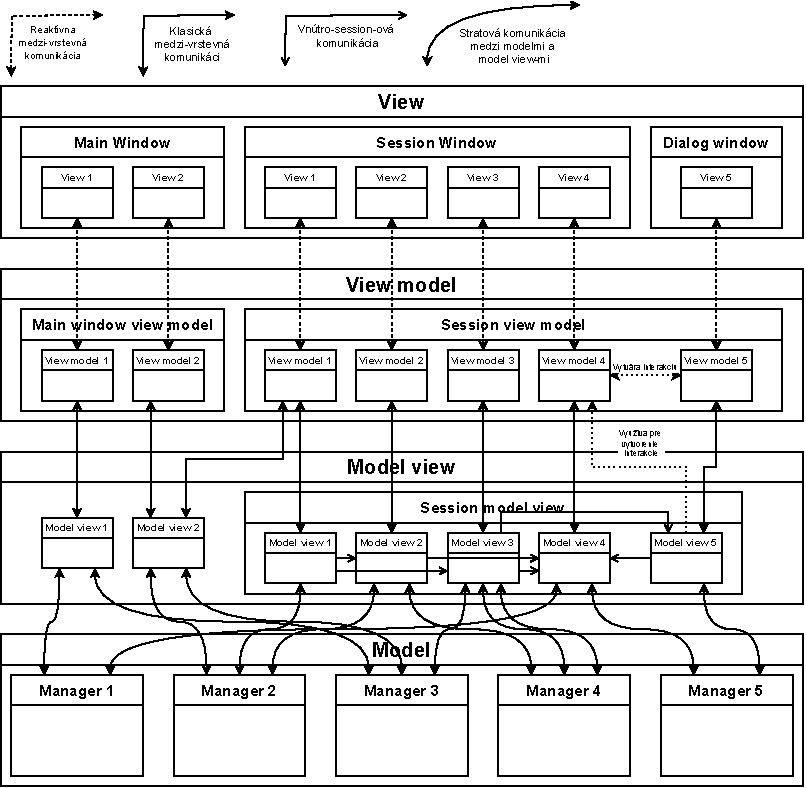
\includegraphics[]{img/horizontalna_struktura}
\caption{Príklad možnej horizontálnej štruktúry aplikácie} 
\label{obr02:horizontalna_struktura}
\end{figure}

\pagebreak

\section{Session-y + \textit{hlavné okno}}\label{Sessions}

Aplikácia, či už z vizuálneho, logického či implementačného hladiska je rozdelená do tzv. \textit{session}-ov. Session-y sú najväčšie stavebné jednotky z ktorých každá predstavuje jedinečný mechanizmus dodávaný aplikáciou. Session-ov (aj rovnakého druhu) môže byť v aplikácii pustených viacero naraz.  

Session-y sú vytvárané v \textit{hlavnom okne}.



